% ==============================================================================
% This file is part of the "LaTeX template for writing the Final Degree Work
% report". It has been developed to aid the students of the Bachelor's Degree in
% Video Game Design and Development at the Jaume I University.
%
% (c) 2019 Sergio Barrachina Mir and José Vte. Martí Avilés
%
% The template can be used and distributed under the next license:
%  Creative Commons Attribution-NonCommercial-ShareAlike (CC BY-NC-SA)
%  http://creativecommons.org/licenses/by-nc-sa/3.0/
%  http://creativecommons.org/licenses/by-nc-sa/3.0/legalcode
%
% Atom editor configuration follows:
% !TEX root = ./report.tex
% !TeX spellcheck = en-US
% ==============================================================================

\chapter{Planning and resources evaluation}

\minitoc{}

\bigskip{}

The following tasks would be performed iteratively (see Figure~\ref{fig:tasks}):
First, a simple game will be developed to serve as an example case for the model. 
Then, different pre-programmed NPC behaviors will be used as training examples. Using ML Agents, a neural network will be trained to imitate that NPC. The results obtained in each training session will be analized to extract conclusions on why the trained network performs well or not. Then, we will start again with other NPC or neural network structures, until we gather enough data to extract conclusions and standardize a general model.

\begin{figure}
  \centering
		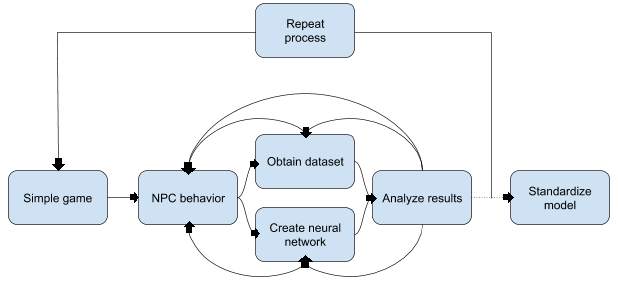
\includegraphics[width=.9\textwidth]{img/taskGraph.png}
  \caption{Planning graph}
  \label{fig:tasks}
\end{figure}

\section{Planning}

\begin{figure}
  \centering
		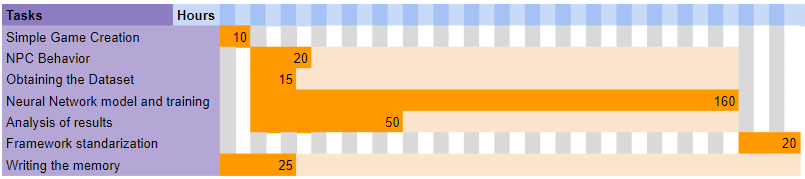
\includegraphics[width=.9\textwidth]{img/ganttChart.png}
  \caption{Initial planning}
  \label{fig:planchart}
\end{figure}

The simple game programming is expected to take 10 hours of work. Then, several neural networks will be trained iteratively and analyzed. At the end, we expect to standardize a framework for more complex behaviors.
The memory will be written during all the process.

\subsection{Simple game creation}

Using Unity3D, the first step is to program a simple 3D video game that serves as the basis for this project.

The game devised is of the “shooter” type, although in this case it could be compared more with a “point-and-click”. The player can only move the view with the mouse and "shoot" by clicking. The game scenario would be very simple to facilitate training (see Figure~\ref{fig:ingame})

\begin{figure}[h]
  \centering
		
\includegraphics[width=.9\textwidth]{img/inGame.png}
  \caption{Actual screenshot of the final game}
  \label{fig:ingame}
\end{figure}

The game screen would have a ratio of 16:9. In this image, the lighter colors correspond to the background and the black with the "enemies" to which you must click. To ease debugging, there would be a white point to represent the sight, which must be aligned with the target to be shot. The agent would receive a visual observation (with no GUI elements) as input.

Like in most shooters, the enemies would have a fixed shape, but the size they look would depend on their distance and inclination with respect to the player, but in this case they would not move. They disappear by clicking over them, and after a few seconds a new enemy appears in another position (the number of enemies will be limited).
The player, when moving the mouse, would move the camera by way of rotation: the sight remains static in the center of the image but the rest of the elements move in the opposite direction of the mouse movement. In the case of vertical movements, the rotation has stops at the zenith and nadir angles, so that you cannot see “upside down”.

\subsection{NPC Behavior}
\label{sec:npcbehavior}

Within the same game, a very simple NPC will be programmed with sensors (rays or colliders) that can play games from the previously described game in random conditions. There are many parameters that could define the behavior of different bots, some examples are:
\begin{itemize}
 \item Reaction time
 \item Speed to which the mouse moves
 \item How many clicks are made on an enemy
 \item Precision of its movements
 \item "Tics" (for example, sudden changes in direction)
 \item Movements made when not seeing enemies
 \item Order in which you select enemies from the same screen
\end{itemize}

In addition, to represent the randomness that real human behavior would entail, each behavior would have a range of imperfection, which could be represented with more parameters such as a random range or a standard deviation.

The bot, unlike the one we intend to create to imitate him, would receive information directly from the stage with sensors such as lightning or a frontal collider that detects collisions with the enemies he has in front of him.

\subsection{Obtaining the Dataset}

Since we intend to imitate a behavior based on the premise that the one who performs it could be a human, the dataset to train must be composed of the information that a human could have of a game: what is seen at each moment, what he has seen in the previous instant and the actions he has performed in that previous instant. With all these data, the action to be performed at this precise moment would be obtained.

The fact of receiving previous information allows to model behaviors with reaction times: it is impossible for a human to react in a frame. The actions allow the movements to have coherence: there could be an interval in which no enemies were seen on the screen, remembering the previous actions you could know if it was moving to the left, the right or it was still.

To obtain this data, it would be necessary to run the game (having the previous bot playing it) and save each of the images, in addition to the inputs that are being made (in Unity, this can be found in “Input.GetAxis” in the case of the movement, and in “Input GetMouseButton or GetMouseButtonDown” in the case of clicks). The Inputs could be saved in a text file, a table or a csv file.

To save the frames, RenderTextures are obtained from the main camera, “Image. EncodeToPNG()” is used to format the image and certain functions of the File class to save files (such as WriteAllBytes). Each frame and input would be assigned a numerical code to obtain them together. Saving files would be executed in LateUpdate(), which is recommended as it is executed after the update of each frame and before the next.

\subsection{Neural network model and training}

Training the neural networks is what takes most of the time. This process includes tuning parameters, designing and balancing rewards and the training itself. In this part of the process some methods to model the behaviors of the NPCs described in section ~\ref{sec:npcbehavior} are designed.

The proposed neural network, in simple terms, is a classification network~\cite{clasnn}: it receives images (and previous actions) as input and returns the action (or actions) to be performed in the current frame.

The input consists of the current frame, a certain number of previous frames and the actions performed on those previous frames. These 3 elements are subjected to convolutions~\footnote{Convolution is a mathematical operation on two functions that produces a third function expressing how the shape of one is modified by the other.} separately (or other kind of compressions) to simplify the information. This information is then processed in a simple network with at least one hidden layer, returning as output the expected action of the current frame, composed of: mouse click (true or false), horizontal and vertical (these last 2 are normalized values representing the speed of movement in the 2 axes, that is, the movement of the mouse). Simpler neural networks could have different architectures, inputs or outputs.

Since in ML Agents all the actions have to be coherent (either discrete or continuous) and the mouse movement needs to be continuous, discrete actions~\footnote{In ML Agents, continuous actions are float numbers. Discrete actions are expressed as an integer, where each possible integer represents a different action.} (clicks or keyboard inputs) would be expressed as a probability of performing it (from 0 to 1).

To train the network, it will be fed with previous frames and actions, the returned action will be compared with the real one that has been performed in that frame, and the error corrected using gradient descent~\cite{mlagents}.


\subsection{Analysis of results}

Once the neural network is trained, it is necessary to incorporate it into Unity so that it can play games and receive inputs in real time.

A first way to check the quality of the behavior generated is visually: the neural network must not only show more or less “intelligent” actions, but must resemble the original. If the behavior doesn’t look anything like the original in all cases, it would be discarded.

If they seem similar, we would make graphs with the actions performed in time (x = time, y = mouse speed on an axis) for each of the 3 actions in order to check if both the reactions and the speed of the movements fall within the range of imprecision that we have defined. From multiple simulations in the same conditions, we could know if the behavior is really similar or not.

After obtaining a result, we would either try to improve it by changing the dataset or the network structure; or repeat the process with another different NPC.

\subsection{Framework standardization}

In the case that we succeed in obtaining similar behaviors (for one or more agents with different behaviors), the next step would be to standardize this method to be able to apply it to more complex games, in which the image has many more elements or there are many more actions available. In that step we would discuss issues such as the feasibility of the model, the accuracy of the results, the cost of training in other cases or the differences between the neural networks in each case (number of layers and neurons per layer).

Also, whether the trained agents imitate the behaviours well or not, we would discuss why that techniques do or do not solve well the imitation problem and what could be done to improve the results.

\section{Resource Evaluation}

The development is intended to be done in an average home PC, but as stated in section~\ref{sec:initialstate} it would be better if a laboratory could be used in parallel. It could be done in reasonable amounts of time (1-4 hours of training per model) while also covering other tasks in parallel.

The only economic cost would be the energy spent in training the neural networks, which could be little high but viable.

In order to execute any of the trained models that were saved in this project, the only requirement is using \textbf{Unity 3D 2019.2.12.f1}. However, to train other neural networks the following requirements must be met:

\begin{itemize}
 \item Python 3.6
 \item Tensorflow 1.15
 \item mlagents 0.11
 \item keras 2.3.1
\end{itemize}

These other requeriments are optional if the training is executed CPU-only, but needed to speed up the process by using GPU:

\begin{itemize}
 \item Cuda 10.0
 \item CuDNN 7.6.5
\end{itemize}

To end with, the system used to train the models has these specifications. They are not a minimum requirement, but can be used as a reference point:

\begin{itemize}
 \item OS: Windows 10
 \item CPU: Intel Core i7-4790
 \item GPU: NVIDIA GeForce GTX 1050
 \item RAM: 24 GB
\end{itemize}
